\section{Direct solution method}%
\label{sec:direct_solution_method}
In this section,
we present the \emph{direct method} for solving linear systems of the form~\eqref{eq:linear_system}
with a general invertible matrix~$\mat A \in \real^{n \times n}$.
The direct method can be decomposed into three steps:
\begin{itemize}
    \item
        First calculate the so-called $\mat L \mat U$ decomposition of $\mat A$,
        i.e.\ find an upper triangular matrix~$\mat U$ and a \emph{unit} lower triangular matrix~$\mat L$ such that
        \(
            \mat A = \mat L \mat U.
        \)
        A unit lower triangular matrix is a lower triangular matrix with only ones on the diagonal.

    \item
        Then solve
        \(
            \mat L \vect y = \vect b
        \)
         using a method called \emph{forward substitution}.

    \item
        Finally, solve
        \(
            \mat U \vect x = \vect y
        \)
         using a method called \emph{backward substitution}.
\end{itemize}
By construction, the solution $\vect x$ thus obtained is a solution to~\eqref{eq:linear_system}.
Indeed, we have that
\[
    \mat A \vect x = \mat L \mat U \vect x = \mat L \vect y = \vect b.
\]

\subsection{LU decomposition}%
\label{sub:lu_decomposition}

In this section,
we first discuss the existence and uniqueness of the $\mat L \mat U$ factorization.
We then describe a numerical algorithm for calculating the factors $\mat L$ and $\mat U$,
based on \emph{Gaussian elimination}.

\subsubsection*{Existence and uniqueness of the decomposition}%
We present a necessary and sufficient condition for the existence of a unique $\mat L \mat U$ decomposition of a matrix.
To this end, we define the principal submatrix of order $i$ of a matrix $\mat A \in \real^{n \times n}$
as the matrix $\mat A_i = \mat A[1:i, 1:i]$, in Julia notation.

\begin{proposition}
    \label{proposition:linear_existence_lu}
    The $\mat L \mat U$ factorization of a matrix $\mat A \in \real^{n \times n}$,
    with $\mat L$ unit lower triangular and $\mat U$ upper triangular,
    exists and is unique if and only if
    the principal submatrices of $\mat A$ of all orders are nonsingular.
\end{proposition}
\begin{proof}
    We prove only the ``if'' direction; see~\cite[Theorem 3.4]{MR2265914} for the ``only if'' implication.

    The statement is clear if $n = 1$.
    Reasoning by induction,
    we assume that the result is proved up to $n - 1$.
    Since the matrix $\mat A_{n-1}$ and all its principal submatrices are nonsingular by assumption,
    it holds that $\mat A_{n-1} = \mat L_{n-1} \mat U_{n-1}$
    for a unit lower triangular matrix $\mat L_{n-1}$ and an upper triangular matrix $\mat U_{n-1}$.
    These two matrices are nonsingular,
    for if either of them were singular then the product $\mat A_{n-1} = \mat L_{n-1} \mat U_{n-1}$ would be singular as well.
    Let us decompose~$\mat A$ as follows:
    \[
        \mat A =
        \begin{pmatrix}
            \mat A_{n-1} & \vect c \\
            \vect d^\t & a_{nn}
        \end{pmatrix}.
    \]
    Let $\vect \ell$ and $\vect u$ denote the solutions to $\mat L_{n-1} \vect u = \vect c$ and $\mat U_{n-1}^\t \vect \ell = \vect d$.
    These solutions exist and are unique,
    because the matrices $\mat L_{n-1}$ and $\mat U_{n-1}$ are nonsingular.
    Letting $u_{nn} = a_{nn} - (\vect \ell^\t \vect u)^{-1}$,
    we check that $\mat A$ factorizes as
    \[
        \begin{pmatrix}
            \mat A_{n-1} & \vect c \\
            \vect d^\t & a_{nn}
        \end{pmatrix}
        =
        \begin{pmatrix}
            \mat L_{n-1} & \vect 0_{n-1} \\
            \vect \ell^\t & 1
        \end{pmatrix}
        \begin{pmatrix}
            \mat U_{n-1} & \vect u \\
            \vect 0_{n-1}^\t & u_{nn}
        \end{pmatrix}.
    \]
    This completes the proof of the existence of the decomposition.
    The uniqueness of the factors follows from the uniqueness of $\vect \ell$, $\vect u$ and $u_{nn}$.
\end{proof}

% \begin{remark}
%     In fact,
%     the reasoning in the proof of~\cref{proposition:linear_existence_lu} can also be employed to show uniqueness of the $\mat L \mat U$ decomposition.
%     The advantage of our approach in the proof of \cref{proposition:linear_uniqueness_lu} is that this approach also implies,
%     as a byproduct, that the iterative procedure for calculating the $\mat L \mat U$ decomposition is well-defined.
% \end{remark}

\cref{proposition:linear_existence_lu} raises the following question:
are there classes of matrices whose principal matrices are all nonsingular?
The answer is positive, and we mention,
as an important example, the class of positive definite matrices.
Proving this is the aim of \cref{exercise:linear_positive_definite_matrix_nonsingular_principal_components}.

\subsection*{Gaussian elimination algorithm for computing $\mat L$ and $\mat U$}%
\label{sub:gaussian_elimination_algorithm_for_computing_mat_l_and_mat_u_}

So far we have presented a condition under which the $\mat L \mat U$ decomposition of a matrix exists and is unique,
but not a practical method for calculating the matrices $\mat L$ and $\mat U$.
We describe in this section an algorithm,
known as \emph{Gaussian elimination},
for calculating the $\mat L \mat U$ decomposition of a matrix.
We begin by introducing the concept of \emph{Gaussian transformation}.
\begin{definition}
    A Gaussian transformation is a matrix of the form $\mat M_k = \mat I - \vect c^{(k)} \vect e_k^\t$,
    where~$\vect e_k$ is the column vector with entry at index $k$ equal to 1 and all the other entries equal to zero,
    and $\vect c^{(k)}$ is a column vector of the following form:
    \[
        \vect c^{(k)} =
        \begin{pmatrix}
            0 & 0 & \dots & 0 & c^{(k)}_{k+1} & c^{(k)}_{k+2} & \dots & c^{(k)}_n
        \end{pmatrix}^\t.
    \]
\end{definition}

The action of a Gaussian transformation $\mat M_k$ left-multiplying a matrix $\mat A \in \real^{n \times n}$ is
to replace the rows from index $k + 1$ to index $n$ by a linear combination involving themselves and the $k$-th row.
To see this, let us denote by $(\vect r^{(i)})_{1 \leq i \leq n}$ the rows of a matrix $\mat T \in \real^{n \times n}$.
Then, we have
\[
    \mat M_k \mat T
    = \bigl(\mat I - \vect c^{(k)} \vect e_k^\t\bigr) \mat T
    =
    \begin{pmatrix}
        1   \\
      & 1  \\
         & &  \ddots \\
        & & & 1 & & & \\
        & & & - c^{(k)}_{k+1} & 1  \\
        & & & \vdots & & \ddots \\
        & & & - c^{(k)}_n & & & 1 \\
    \end{pmatrix}
    \begin{pmatrix}
        \vect r^{(1)} \\
        \vect r^{(2)} \\
        \vdots \\
        \vect r^{(k)} \\
        \vect r^{(k+1)} \\
        \vdots \\
        \vect r^{(n)}
    \end{pmatrix}
    =
    \begin{pmatrix}
        \vect r^{(1)} \\
        \vect r^{(2)} \\
        \vdots \\
        \vect r^{(k)} \\
        \vect r^{(k+1)} - c^{(k)}_{k+1} \vect r^{(k)} \\
        \vdots \\
        \vect r^{(n)} - c^{(k)}_{n} \vect r^{(k)}
    \end{pmatrix}
\]
We show in \cref{exercise:inverse_gaussian_transformation} that
the inverse of a Gaussian transformation matrix is given by
\begin{equation}
    \label{eq:inverse_gaussian_transformation}
    (\mat I - \vect c^{(k)} \vect e_k^\t)^{-1} = \mat I + \vect c^{(k)} \vect e_k^\t.
\end{equation}
The idea of the Gaussian elimination algorithm is to successively left-multiply $\mat A$
with Gaussian transformation matrices $\mat M_1$, then $\mat M_2$, etc.\
appropriately chosen in such a way that the matrix~$\mat A^{(k)}$,
obtained after $k$ iterations,
is upper triangular up to column $k$.
That is to say, the Gaussian transformations are constructed so that
all the entries in columns~1 to~$k$ under the diagonal of the matrix $\mat A^{(k)}$ are equal to zero.
The resulting matrix $\mat A^{(n-1)}$ after $n-1$ iterations is then upper triangular
and satisfies
\[
    \mat A^{(n-1)} = \mat M_{n-1} \dotsc \mat M_1 \mat A.
\]
Rearranging this equation,
we deduce that
\[
    \mat A = (\mat M_1^{-1} \dots \mat M_{n-1}^{-1}) \mat A^{(n-1)}.
\]
The first factor is lower triangular by~\eqref{eq:inverse_gaussian_transformation} and \cref{exercise:linear_product_of_lower_triangular}.
The product in the definition of the matrix $\mat L$ admits a simple explicit expression.
\begin{lemma}
    \label{lemma:linear_inverse_product_gaussian_transformations}
    It holds that
    \begin{equation*}
        % \label{eq:product_inverse}
        \mat M_1^{-1} \dotsb \mat M_{n-1}^{-1}
        = (\mat I + \vect c^{(1)} \vect e_1^\t) \dotsb (\mat I + \vect c^{(n-1)} \vect e_{n-1}^\t)
        = \mat I + \sum_{i=1}^{n-1}  \vect c^{(i)} \vect e_i^\t.
    \end{equation*}
\end{lemma}
\begin{proof}
    Notice that, for $i < j$,
    \[
        \vect c^{(i)} \vect e_i^\t \vect c^{(j)} \vect e_j^\t
        = \vect c^{(i)} (\vect e_i^\t \vect c^{(j)}) \vect e_j^\t
        = \vect c^{(i)} 0 \vect e_j^\t = 0.
    \]
    The statement then follows easily by expanding the product.
\end{proof}
A corollary of~\cref{lemma:linear_inverse_product_gaussian_transformations} is that all the diagonal entries of the lower triangular matrix $\mat L$ are equal to 1;
the matrix $\mat L$ is \emph{unit lower triangular}.
The full expression of the matrix $\mat L$ given the Gaussian transformations is
\begin{equation}
    \label{eq:linear_matrix_L}
    \mat L
    = \mat I +
    \begin{pmatrix}
        \vect c^{(1)} & \hdots & \vect c^{(n)} & \vect 0_n
    \end{pmatrix}
    =
    \begin{pmatrix}
        1 & \\
        c^{(1)}_2 & 1 \\
        c^{(1)}_3 & c^{(2)}_3 & 1 \\
        c^{(1)}_4 & c^{(2)}_4 & c^{(3)}_4 &  1 \\
        \vdots & \vdots & \vdots & & \ddots \\
        c^{(1)}_n & c^{(2)}_n & c^{(3)}_n & \hdots & c^{(n-1)}_n & 1 \\
    \end{pmatrix}
\end{equation}
Therefore, the Gaussian elimination algorithms, if all the steps are well-defined,
correctly gives the $\mat L \mat U$ factorization of the matrix $\mat A$.
% In practical implementations, therefore,
% these diagonal entries can be omitted and the matrices $\mat L$ and $\mat U$ can be stored within the same matrix.
Of course, the success of the strategy outlined above for the calculation of the $\mat L \mat U$ factorization hinges on
the existence of an appropriate Gaussian transformation at each iteration.
It is not difficult to show that,
if the $(k+1)$-th diagonal entry of the matrix $\mat A^{(k)}$ is nonzero for all~$k \in \{1, \dotsc, n-2\}$,
then the Gaussian transformation matrices exist and are uniquely defined.
\begin{lemma}
    \label{lemma:linear_expression_gaussian_transformations}
    Assume that $\mat A^{(k)}$ is upper triangular up to column $k$ included,
    with $k \leq n-2$.
    If~$a^{(k)}_{k+1,k+1} > 0$,
    then there is a unique Gaussian transformation matrix $\mat M_{k+1}$ such that $\mat M_{k+1} \mat A^{(k)}$ is upper triangular up to column $k + 1$.
    This transformation matrix is given by $\mat I - \vect c^{(k+1)} \vect e_{k+1}^\t$, where
    \[
        \vect c^{(k+1)} =
        \begin{pmatrix}
            0 & 0 & \dots & 0 & \frac{a^{(k)}_{k+2,k+1}}{a^{(k)}_{k+1,k+1}} & \frac{a^{(k)}_{k+3,k+1}}{a^{(k)}_{k+1,k+1}} & \dots & \frac{a^{(k)}_{n,k+1}}{a^{(k)}_{k+1,k+1}}
        \end{pmatrix}^\t.
    \]
\end{lemma}
\begin{proof}
    We perform the multiplication explicitly.
    Denoting denote by $(\vect r^{(i)}){1 \leq i \leq n}$ the rows of $\mat A^{(k)}$,
    we have
    \[
        \mat M_{k + 1} \mat A^{(k)}
        =
        \begin{pmatrix}
                1   \\
          & 1  \\
          & &  \ddots \\
          & & & 1 & & & \\
          & & & - c^{(k+1)}_{k+2} & 1  \\
          & & & \vdots & & \ddots \\
          & & & - c^{(k+1)}_n & & & 1 \\
        \end{pmatrix}
        \begin{pmatrix}
            \vect r^{(1)} \\
            \vect r^{(2)} \\
            \vdots \\
            \vect r^{(k+1)} \\
            \vect r^{(k+2)} \\
            \vdots \\
            \vect r^{(n)}
        \end{pmatrix}
        =
        \begin{pmatrix}
            \vect r^{(1)} \\
            \vect r^{(2)} \\
            \vdots \\
            \vect r^{(k+1)} \\
            \vect r^{(k+2)} - c^{(k+1)}_{k+2} \vect r^{(k+1)} \\
            \vdots \\
            \vect r^{(n)} - c^{(k+1)}_{n} \vect r^{(k+1)}
        \end{pmatrix}.
    \]
    We need to show that the matrix on the right-hand side is upper triangular up to column $k+1$ included.
    This is clear by definition of $\vect c^{(k+1)}$ and from the fact that $\mat A^{(k)}$ is upper triangular up to column $k$ by assumption.
\end{proof}

The diagonal elements $a^{(k)}_{k+1,k+1}$, where $k \in \{0, \dots, n-2 \}$, are called the pivots.
We now prove that,
if an invertible matrix $\mat A$ admits an $\mat L \mat U$ factorization,
then the pivots are necessarily nonzero and the Gaussian elimination algorithm is successful.
\begin{proposition}
    [Gaussian elimination works~\moreinfo]
    \label{proposition:linear_uniqueness_lu}
    If $\mat A$ is invertible and admits an $\mat L \mat U$  factorization,
    then the Gaussian elimination algorithm is well-defined and successfully terminates.
\end{proposition}
\begin{proof}
    We denote by $\vect c^{(1)}, \dotsc, \vect c^{(n-1)},$ the columns of the matrix $\mat L - \mat I$.
    Then the matrices given by $\mat M_k = \mat I - \vect c^{(k)} \vect e_{k}^\t$,
    for $k \in \{1, \dotsc, n-1 \}$,
    are Gaussian transformations and it holds that
    \[
        \mat L = \mat M_1^{-1} \dotsb  \mat M_{n-1}^{-1}
    \]
    in view of \cref{lemma:linear_inverse_product_gaussian_transformations}.
    Since $\mat A = \mat L \mat U$ by assumption,
    the result of the product
    \[
        \mat M_{n-1} \dotsb \mat M_1 \mat A = \mat U
    \]
    is upper triangular.
    Let us use the notation $\mat A^{(k)} = \mat M_{k} \dotsb \mat M_1 \mat A$.
    Our goal is to show that the matrices~$\mat M_1, \dotsc, \mat M_{n-1}$ are the same as those obtained by the Gaussian elimination algorithm.

    Of all the Gaussian transformations $\mat M_1, \dotsc, \mat M_{n-1}$,
    only $\mat M_1$ acts on the second row of the matrix it multiplies.
    Therefore, the entry $(2, 1)$ of~$\mat U$ coincides with the entry $(2, 1)$ of $\mat A^{(1)}$,
    which implies that $a^{(1)}_{2,1} = 0$.
    % and since $u_{2,1} = 0$ we deduce that $a_{21} - c^{(1)}_2 a_{11} = 0$.
    Then notice that $a^{(k)}_{3,1} = a^{(1)}_{3, 1}$ for all $k \geq 1$,
    because the entry $(3, 1)$ of the matrix $\mat M_2 \mat A^{(1)}$ is given by $a^{(1)}_{3,1} - c^{(2)}_3 a^{(1)}_{2,1} = a^{(1)}_{3,1}$,
    and all the other transformation matrices $\mat M_3, \dotsc, \mat M_{n-1}$ leave the third row invariant.
    Consequently, it holds that $a^{(1)}_{3,1} = u_{3,1} = 0$.
    Continuing in this manner,
    we deduce that $\mat A^{(1)}$ is upper triangular in the first column and that,
    since $\mat A$ is invertible by assumption,
    the first pivot~$a_{11}$ is nonzero.
    Since this pivot is nonzero,
    the matrix $\mat M_1$ is uniquely defined by~\cref{lemma:linear_expression_gaussian_transformations}.

    The reasoning can then be repeated with other columns,
    in order to deduce that $\mat A^{(k)}$ is upper triangular up to column $k$ and that all the pivots $a^{(k-1)}_{kk}$ are nonzero.
    Therefore, all the Gaussian transformation matrices are uniquely defined given~\cref{lemma:linear_expression_gaussian_transformations}.
    % Since this uniquely defines the Gaussian transformations by \cref{lemma:linear_expression_gaussian_transformations},
    % we conclude that $\mat L$ is unique, and therefore $\mat U = \mat L^{-1} \mat A$ is also unique.
\end{proof}


\subsection*{Computer implementation}%
\label{sub:computer_implementation}

The Gaussian elimination procedure is summarized as follows.

% \begin{algorithm}
% \caption{$\mat L \mat U$ factorization algorithm}%
% \label{algo:factorization_algorithm}%
\begin{algorithmic}
\State $\mat A^{(0)} \gets \mat A, \mat L \gets \mat I$
\For{$i \in \{1, \dotsc, n-1\}$}
    \State Construct $\mat M_{i}$ as in~\cref{lemma:linear_expression_gaussian_transformations}.
    \State $\mat A^{(i)} \gets \mat M_{i} \mat A^{(i-1)}, \mat L \gets \mat \mat \mat L \mat M_i^{-1}$
\EndFor
\State $\mat U \gets \mat A^{(n-1)}$.
\end{algorithmic}
% \end{algorithm}

In practice, it is not necessary to explicitly create the Gaussian transformation matrices,
or to perform full matrix multiplications.
A more realistic version of the algorithm in Julia is given below.
The code exploits the relation~\eqref{eq:linear_matrix_L} between $\mat L$ and the parameters of the Gaussian transformations.
\begin{minted}[xleftmargin=\parindent, linenos, mathescape]{julia}
 # A is an invertible matrix of size n x n
 L = [i == j ? 1.0 : 0.0 for i in 1:n, j in 1:n]
 U = copy(A)
 for i in 1:n-1
     for r in i+1:n
         U[i, i] == 0 && error("Pivotal entry is zero!")
         ratio = U[r, i] / U[i, i]
         L[r, i] = ratio
         U[r, i:end] -= U[i, i:end] * ratio
     end
 end
 # L is unit lower triangular and U is upper triangular
\end{minted}

\subsubsection*{Computational cost}%
\label{ssub:computational_cost}
The computational cost of the algorithm,
measured as the number of floating point operations (flops) required,
is dominated by the Gaussian transformations,
in line 9 in the above code.
All the other operations amount to a computational cost scaling as $\mathcal O(n^2)$,
which is negligible compared to the cost of the $\mat L \mat U$ factorization when $n$ is large.
This factorization requires
\[
    \overbrace{2\times}^{\text{\julia{-} and \julia{*}}} \underbrace{\sum_{i=1}^{n-1}}_{\julia{for i in 1:n-1}} \overbrace{(n - i)}^{\julia{for r in i+1:n}} \underbrace{(n - i + 1)}_{\text{indices \julia{[i:end]}}} \quad \mathrm{flops}
    = \frac{2}{3} n^3 + \mathcal O(n^2) \quad \mathrm{flops}.
\]

\subsection{Backward and forward substitution}%
\label{sub:backward_and_forward_substitution}
Once the $\mat L \mat U$ factorization has been completed,
the solution to the linear system can be obtained by first using forward, and then backward substitution,
which are just bespoke methods for solving linear systems with lower and upper triangular matrices, respectively.
Let us consider the case of a lower triangular system:
\[
    \mat L \vect y = \vect b
\]
Notice that the unknown $y_1$ may be obtained from the first equation of the system.
Then, since $y_1$ is known, the value of $y_2$ can be obtained from the second equation, etc.
A simple implementation of this algorithm is as follows:
\begin{minted}{julia}
    # L is unit lower triangular
    y = copy(b)
    for i in 2:n
        for j in 1:i-1
            y[i] -= L[i, j] * y[j]
        end
    end
\end{minted}

\subsection{Gaussian elimination with pivoting~\moreinfo}%
\label{sub:pivoting}
The Gaussian elimination algorithm that
we presented in \cref{sub:lu_decomposition} relies on the existence of an $\mat L \mat U$ factorization.
In practice,
this assumption may not be satisfied,
and in this case a modified algorithm,
called Gaussian elimination \emph{with pivoting},
is required.

In fact, pivoting is useful even if the usual $\mat L \mat U$ decomposition of $\mat A$ exists,
as it enables to reduce the condition number of the matrices matrices~$\mat L$ and~$\mat U$.
There are two types of pivoting:
partial pivoting, where only the rows are rearranged through a permutation at each iteration,
and complete pivoting, where both the rows and the columns are rearranged at each iteration.

Showing rigorously why pivoting is useful is beyond the scope of this course.
In this section, we only present the partial pivoting method.
Its influence on the condition number of the factors $\mat L$ and $\mat U$ is studied empirically in \cref{exercise:linear_lu_with_partial_pivoting}.
It is useful at this point to introduce the concept of a row permutation matrix.

\subsubsection*{Row permutation matrix}%
\begin{definition}
    \label{definition:row_permutation_matrix}%
    Let $\sigma : \{1, \dotsc, n\} \to \{1, \dotsc, n\}$ be a permutation,\
    i.e.\ a bijection on the set~$\{1, \dotsc, n\}$.
    The row permutation matrix associated with $\sigma$ is the matrix with entries
    \[
        p_{ij} =
        \begin{cases}
            1 & \text{if $i = \sigma(j)$,} \\
            0 & \text{otherwise.}
        \end{cases}
    \]
\end{definition}
When a row permutation $\mat P$ left-multiplies a matrix $\mat B \in \real^{n \times n}$,
row~$i$ of matrix $\mat B$ is moved to row index $\sigma(i)$ in the resulting matrix,
for all $i \in \{1, \dots, n\}$.
A permutation matrix has a single entry equal to~1 per row and per column,
and its inverse coincides with its transpose:~$\mat P^{-1} = \mat P^\t$.

\subsubsection*{Partial pivoting}%
Gaussian elimination with partial pivoting applies for any invertible matrix $\mat A$,
and it outputs 3 matrices: a row permutation $\mat P$, a unit triangular matrix $\mat L$,
and an upper triangular matrix $\mat U$.
These are related by the relation
\[
    \mat P \mat A = \mat L \mat U.
\]
This is sometimes called a $\mat P \mat L \mat U$ decomposition of the matrix $\mat A$.
It is not unique in general but, unlike the usual $\mat L \mat U$ decomposition,
it always exists provided that $\mat A$ is invertible.
We take this for granted in this course.

The idea of partial pivoting is to rearrange the rows at each iteration of the Gaussian elimination procedure in such a manner that
the pivotal entry is as large as possible in absolute value.
One step of the procedure reads
\begin{equation}
    \label{eq:step_partial_pivoting}
    \mat A^{(k+1)} = \mat M_{k+1} \mat P_{k+1} \mat A^{(k)}.
\end{equation}
Here $\mat P_{k+1}$ is a simple row permutation matrix which,
when acting on $\mat A^{(k)}$,
interchanges row~$k+1$ and row $\ell$,
for some index $\ell \geq k+1$.
The row index $\ell$ is selected in such a way that the absolute value of the pivotal entry,
in position $(k+1, k+1)$ of the product~$\mat P_{k+1} \mat A^{(k)}$, is maximum.
The matrix $\mat M_{k+1}$ is then the unique Gaussian transformation matrix ensuring that~%
$\mat A^{(k+1)}$ is upper triangular up to column~$k+1$,
obtained as in~\cref{lemma:linear_expression_gaussian_transformations}.
The resulting matrix $\mat A^{(n-1)}$ after~$n-1$ steps of the form~\eqref{eq:step_partial_pivoting} is upper triangular and satisfies
\[
    \mat A^{(n-1)} = \mat M_{n-1} \mat P_{n-1} \dotsb \mat M_{1} \mat P_{1} \mat A
    \quad \Leftrightarrow \quad
     \mat A = (\mat M_{n-1} \mat P_{n-1} \dotsb \mat M_{1} \mat P_{1})^{-1} \mat A^{(n-1)}.
\]
The first factor in the decomposition of $\mat A$ is not necessarily lower triangular.
However, using the notation $\mat M = \mat M_{n-1} \mat P_{n-1} \dotsb \mat M_{1} \mat P_{1}$ and $\mat P = \mat P_{n-1} \dotsb \mat P_{1}$,
we have
\begin{equation}
    \label{eq:plu_decomposition}
    \mat P \mat A = \mat P \mat M^{-1} \mat U = (\mat P \mat M^{-1}) \mat U =: \mat L \mat U.
\end{equation}
\Cref{lemma:linear_matrix_l_pivoting} below shows that,
as the notation $\mat L$ suggests,
the matrix $\mat L = (\mat P \mat M^{-1})$ on the right-hand side is indeed lower triangular.
Before stating and proving the lemma,
we note that $\mat P$ is a row permutation matrix,
and so the solution to the linear system $\mat A \vect x = \mat b$ can be obtained by solving $\mat L \mat U \vect x = \mat P^\t \vect b$
by forward and backward substitution.
Since $\mat P$ is a very sparse matrix,
the right-hand side~$\mat P^\t \vect b$ can be calculated very efficiently.
\begin{lemma}
    \label{lemma:linear_matrix_l_pivoting}
    The matrix $\mat L = \mat P \mat M^{-1}$ is unit lower triangular
    with all entries bounded in absolute value from above by 1.
    It admits the expression
    \[
        \mat L
        = \mat I
        + (\mat P_{n-1} \dotsb \mat P_{2} \vect c^{(1)}) \vect e_{1}^\t
        + (\mat P_{n-1} \dotsb \mat P_{3} \vect c^{(2)}) \vect e_{2}^\t
        + \dotsb
        + (\mat P_{n-1} \vect c^{(n-2)}) \vect e_{n-2}^\t
        + \vect c^{(n-1)} \vect e_{n-1}^\t.
    \]
\end{lemma}
\begin{proof}
    Let $\mat M^{(k)} = \mat M_{k} \mat P_{k} \dotsb \mat M_{1} \mat P_{1}$ and $\mat P^{(k)} = \mat P_{k} \dotsb \mat P_{1}$.
    It is sufficient to show that
    \begin{equation}
        \label{eq:linear_lower_triangular_l}
        \mat P^{(k)} \bigl( \mat M^{(k)} \bigr)^{-1}
        = \mat I
        + (\mat P_{k} \dotsb \mat P_{2} \vect c^{(1)}) \vect e_{1}^\t
        + (\mat P_{k} \dotsb \mat P_{3} \vect c^{(2)}) \vect e_{2}^\t
        + \dotsb
        + (\mat P_{k} \vect c^{(k-1)}) \vect e_{k-1}^\t
        + \vect c^{(k)} \vect e_{k}^\t
    \end{equation}
    for all $k \in \{1, \dotsc, n-1 \}$.
    The statement is clear for $k = 1$,
    and we assume by induction that it is true up to~$k-1$.
    Then notice that
    \begin{align*}
        \mat P^{(k)} \bigl( \mat M^{(k)} \bigr)^{-1}
        &= \mat P_{k} \left( \mat P^{(k-1)} \bigl( \mat M^{(k-1)} \bigr)^{-1} \right) \mat P_k^{-1} \mat M_k^{-1} \\
        &= \mat P_{k} \Bigl( \mat I
        + (\mat P_{k-1} \dotsb \mat P_{2} \vect c^{(1)}) \vect e_{1}^\t
        + \dotsb
        + (\mat P_{k-1} \vect c^{(k-2)}) \vect e_{k-2}^\t
        + \vect c^{(k-1)} \vect e_{k-1}^\t \Bigr) \mat P_k^{-1} \mat M_k^{-1} \\
        &= \Bigl( \mat I
        + (\mat P_k \mat P_{k-1} \dotsb \mat P_{2} \vect c^{(1)}) \vect e_{1}^\t
        + \dotsb
        + (\mat P_k \mat P_{k-1} \vect c^{(k-2)}) \vect e_{k-2}^\t
        + (\mat P_k \vect c^{(k-1)}) \vect e_{k-1}^\t \Bigr) \mat M_k^{-1}.
    \end{align*}
    In the last equality,
    we used that $\vect e_{i}^\t \mat P_k^{-1} = (\mat P_k \vect e_i)^\t = \vect e_i^\t$ for all $i \in \{1, \dotsc, k-1\}$,
    because the row permutation $\mat P_k$ does not affect rows~$1$ to~$k-1$.
    Using the expression $\mat M_k^{-1} = \mat I + \vect c^{(k)} \vect e_k^\t$,
    expanding the product and noting that $\vect e_j^\t \vect c^{(k)} = 0$ if $j \leq k$,
    we obtain~\eqref{eq:linear_lower_triangular_l}.
    The statement that the entries are bounded in absolute value from above by 1 follows from the choice of the pivot at each iteration.
\end{proof}
The expression of $\mat L$ in \cref{lemma:linear_matrix_l_pivoting} suggests the iterative procedure given in~\cref{algo:LU_decomposition_with_partial_pivoting} for performing the $\mat L \mat U$ factorization with partial pivoting.
A Julia implementation of this algorithm is presented in~\cref{julia:lu_factorization_with_pivoting}.
\begin{algorithm}
\caption{$\mat L \mat U$ decomposition with partial pivoting}%
\label{algo:LU_decomposition_with_partial_pivoting}%
\begin{algorithmic}
\State Assign $\mat A^{(0)} \gets \mat A$ and $\mat P \gets \mat I$
\For{$i \in \{1, \dotsc, n-1\}$}
    \State Find the row index $k \geq i$ such that $\mat A^{(i-1)}_{k,i}$ is maximum in absolute value.
    \State Interchange the rows $i$ and $k$ of matrices $\mat A^{(i-1)}$ and $\mat P$, and of vectors $\vect c^{(1)}, \dotsc, \vect c^{(i-1)}$.
    \State Construct $\mat M_{i}$ with corresponding column vector $\vect c^{(i)}$ as in~\cref{lemma:linear_expression_gaussian_transformations}.
    \State Assign $\mat A^{(i)} \gets \mat M_{i} \mat A^{(i-1)}$
\EndFor
\State Assign $\mat U \gets \mat A^{(n-1)}$.
\State Assign $\mat L \gets \mat I + \begin{pmatrix} \vect c^{(1)} & \hdots & \vect c^{(n-1)} & \vect 0_n \end{pmatrix}$.
\end{algorithmic}
\end{algorithm}

\begin{code}
\begin{minted}[fontsize=\footnotesize]{julia}
    # Auxiliary function
    function swap_rows!(i, j, matrices...)
        for M in matrices
            M_row_i = M[i, :]
            M[i, :] = M[j, :]
            M[j, :] = M_row_i
        end
    end

    n = size(A)[1]
    L, U = zeros(n, 0), copy(A)
    P = [i == j ? 1.0 : 0.0 for i in 1:n, j in 1:n]
    for i in 1:n-1
        # Pivoting
        index_row_pivot = i - 1 + argmax(abs.(U[i:end, i]))
        swap_rows!(i, index_row_pivot, U, L, P)

        # Usual Gaussian transformation
        c = [zeros(i-1); 1.0; zeros(n-i)]
        for r in i+1:n
            ratio = U[r, i] / U[i, i]
            c[r] = ratio
            U[r, i:end] -= U[i, i:end] * ratio
        end
        L = [L c]
    end
    L = [L [zeros(n-1); 1.0]]
    # It holds that P*A = L*U
\end{minted}
\caption{%
    $\mat L \mat U$ factorization with partial pivoting.
}%
\label{julia:lu_factorization_with_pivoting}
\end{code}

\begin{remark}
    It is possible to show that,
    if the matrix $\mat A$ is column diagonally dominant in the sense that
    \[
        \forall j \in \{1, \dotsc, n\}, \qquad
        \lvert a_{jj} \rvert \geq \sum_{i=1, i\neq j}^{n} \lvert a_{ij} \rvert,
    \]
    then pivoting does not have an effect:
    at each iteration,
    the best pivot is already on the diagonal.
\end{remark}

\subsection{Direct method for symmetric positive definite matrices}%
\label{sub:direct_method_for_symmetric_positive_definite_matrices}
The $\mat L \mat U$ factorization with partial pivoting applies to any matrix $\mat A \in \real^{n \times n}$ that is invertible.
If~$\mat A$ is symmetric positive definite,
however, it is possible to compute a factorization into lower and upper triangular matrices at half the computational cost,
using the so-called \emph{Cholesky decomposition}.
\begin{lemma}
    [Cholesky decomposition]
    If~$\mat A$ is symmetric positive definite,
    then there exists a lower-triangular matrix $\mat C \in \real^{n \times n}$ such that
    \begin{equation}
        \label{eq:linear_cholesky_decomposition}
        \mat A = \mat C \mat C^\t.
    \end{equation}
    Equation~\eqref{eq:linear_cholesky_decomposition} is called the Cholesky factorization of $\mat A$.
    The matrix $\mat C$ is unique if we require that all its diagonal entries are positive.
\end{lemma}
\begin{proof}
    Since $\mat A$ is positive definite,
    its $\mat L \mat U$ decomposition exists and is unique by~\cref{proposition:linear_uniqueness_lu,proposition:linear_existence_lu}.
    Let $\mat D$ denote the diagonal matrix with the same diagonal as that of $\mat U$.
    Then
    \[
        \mat A = \mat L \mat D \mat (\mat D^{-1} \mat U).
    \]
    Note that the matrix $\mat D^{-1} \mat U$ is unit upper triangular.
    Since $\mat A$ is symmetric,
    we have
    \[
        \mat A = \mat A^\t = (\mat D^{-1} \mat U)^\t (\mat L \mat D)^\t.
    \]
    The first and second factors on the right-hand side are respectively unit lower triangular and upper triangular,
    and so we deduce, by uniqueness of the $\mat L \mat U$ decomposition,
    that $\mat L = (\mat D^{-1} \mat U)^\t$ and $\mat U = (\mat L \mat D)^\t$.
    But then
    \[
        \mat A = \mat L \mat U = \mat L \mat D \mat L^\t = (\mat L \sqrt{\mat D}) (\sqrt{\mat D} \mat L)^\t.
    \]
    Here $\sqrt{\mat D}$ denotes the diagonal matrix whose diagonal entries are obtained by taking the square root of those of $\mat D$,
    which are necessarily positive because $\mat A$ is positive definite.
    This implies the existence of a Cholesky factorization with $\mat C = \mat L \sqrt{\mat D}$.
\end{proof}

\subsubsection*{Calculation of the Choleski factor}%

The matrix $\mat C$ can be calculated from~\eqref{eq:linear_cholesky_decomposition}.
For example, developing the matrix product gives that $a_{1,1} = c_{1, 1}^2$ and so $c_{1, 1} = \sqrt{a_{1,1}}$.
It is then possible to calculate $c_{2,1}$ from the equation~$a_{2, 1} = c_{2, 1} c_{1, 1}$, and so on.
Implementing the Cholesky factorization is the goal of \cref{exercise:linear_cholesky}.

\subsection{Direct methods for banded matrices}%

In applications related to partial differential equations,
the matrix $\mat A \in \real^{n \times n}$ very often has a bandwidth which is small in comparison with $n$.
\begin{definition}
    The bandwidth of a matrix $\mat A \in \real^{n \times n}$ is the smallest number $k \in \nat$ such that
    $a_{ij} = 0$ for all $(i, j) \in \{1, \dotsc, n\}^2$ with $\abs{i - j} > k$.
\end{definition}
It is not difficult to show that,
if $\mat A$ is a matrix with bandwidth $k$,
then so are $\mat L$ and $\mat U$ in the absence of pivoting.
This can be proved by equaling the entries of the product $\mat L \mat U$ with those of the matrix $\mat A$.
We emphasize, however, that the sparsity structure \emph{within} the band of $\mat A$ may be destroyed in $\mat L$ and $\mat U$;
this phenomenon is called \emph{fill-in}.

\subsubsection{Reducing the bandwidth: the Cuthill--McKee algorithm~\moreinfo}%
\label{ssub:reducing_the_bandwidth_the_cuthill_mckee_algorithm}

The computational cost of calculating the $\mat L \mat U$ or Cholesky decomposition of a matrix with bandwidth $k$ scales as $\mathcal O(n k^2)$,
which is much better than the general scaling $\mathcal O(n^3)$ if $k \ll n$.
In applications, the bandwidth $k$ is often related to the matrix size $n$.
For example, if~$\mat A$ arises from the discretization of the Laplacian operator, then $k = \mathcal O(\sqrt{n})$
provided that a good ordering of the vertices is employed.
In this case, the computational cost scales as $\mathcal O(n^2)$.

Since a narrow band is associated with a lower computational cost of the $\mat L \mat U$ decomposition,
it is natural to wonder whether the bandwidth of a matrix $\mat A$ can be reduced.
A possible strategy to this end is to use permutations.
More precisely, is it possible to identify a row permutation matrix $\mat P$ such that
\(
    \mat P \mat A \mat P^\t
\)
has minimal bandwidth?
Given such a matrix,
the solution to the linear system~\eqref{eq:linear_system} can be obtained by first solving $(\mat P \mat A \mat P^\t) \vect y = \mat P b$,
and then letting $\vect x = \mat P^\t \vect y$.

The Cuthill--McKee algorithm is a heuristic method for finding a good,
but sometimes not optimal,
permutation matrix~$\mat P$ in the particular case where $\mat A$ is a \emph{symmetric} matrix.
It is based on the fact that,
to a symmetric matrix~$\mat A$, we can associate a unique undirected graph whose adjacency matrix~$\mat A_*$ has the same sparsity structure as that of $\mat A$,
i.e.\ zeros in the same places.
For any row permutation matrix $\mat P_{\sigma}$ with corresponding permutation~$\sigma\colon \{1, \dotsc, n\} \rightarrow \{1, \dotsc, n\}$ (see \cref{definition:row_permutation_matrix}),
the matrices~$\mat P_{\sigma} \mat A \mat P_{\sigma}^\t$ and~$\mat P_{\sigma} \mat A_* \mat P_{\sigma}^\t$ also have the same sparsity structure.
Therefore, minimizing the bandwidth of~$\mat P_{\sigma} \mat A \mat P_{\sigma}^\t$ is equivalent to minimizing the bandwidth of~$\mat P_{\sigma} \mat A_* \mat P_{\sigma}^\t$.
The key insight for understanding the Cuthill--McKee method is that $\mat P_{\sigma} \mat A_* \mat P_{\sigma}^\t$ is the adjacency matrix of the graph obtained by renumbering the nodes
according to the permutation $\sigma$,
i.e.\ by changing the number of the nodes from~$i$ to~$\sigma(i)$.
Consider, for example,
the following graph and renumbering:

\hspace{-.5cm}
\begin{minipage}{.24\textwidth}
    \begin{tikzpicture}
        \footnotesize
        \path [graphs/.cd, nodes={shape=circle, fill=blue!40, draw=none},  empty nodes]
            graph [spring layout] { A [as=1] -- B [as=2] -- C [as=3] -- D [as=4] -- D [as=4] -- E [as=5] -- F [as=6] -- G [as=7] -- H [as=8] -- A };
    \end{tikzpicture}
\end{minipage}
\hspace{-.5cm}
\begin{minipage}{.48\textwidth}
    \scriptsize%
    \[
        \begin{pmatrix}
            1 & 1 &   &   &   &   &   & {\color{red} 1} \\
            1 & 1 & 1 &   &   &   &   &   \\
              & 1 & 1 & 1 &   &   &   &   \\
              &   & 1 & 1 & 1 &   &   &   \\
              &   &   & 1 & 1 & 1 &   &   \\
              &   &   &   & 1 & 1 & 1 &   \\
              &   &   &   &   & 1 & 1 & 1 \\
            {\color{red} 1} &   &   &   &   &   & 1 & 1 \\
        \end{pmatrix}
        \rightarrow
        \begin{pmatrix}
            1 & 1 & 1 &   &   &   &   &   \\
            1 & 1 &   & 1 &   &   &   &   \\
            1 &   & 1 &   & 1 &   &   &   \\
              & 1 &   & 1 &   & 1 &   &   \\
              &   & 1 &   & 1 &   & 1 &   \\
              &   &   & 1 &   & 1 &   & 1 \\
              &   &   &   & 1 &   & 1 & 1 \\
              &   &   &   &   & 1 & 1 & 1 \\
        \end{pmatrix}
    \]
\end{minipage}
\hspace{1.5cm}
\begin{minipage}{.24\textwidth}
\begin{tikzpicture}
    \footnotesize
    \path [graphs/.cd, nodes={shape=circle, fill=blue!40, draw=none},  empty nodes]
        graph [spring layout] { A [as=1] -- B [as=2]  -- C [as=4]  -- D [as=6] -- E [as=8]  -- F [as=7]  -- G [as=5] -- H [as=3] -- A };
\end{tikzpicture}
\end{minipage}

\vspace{.2cm}
\noindent Here we also wrote the adjacency matrices associated to the graphs.
We assume that the nodes are all self-connected,
although this is not depicted,
and so the diagonal entries of the adjacency matrices are equal to 1.
This renumbering corresponds to the permutation
\begin{align*}
    \begin{pmatrix}
        i:         & 1 & 2 & 3 & 4 & 5 & 6 & 7 & 8 \\
        \sigma(i): & 1 & 2 & 4 & 6 & 8 & 7 & 5 & 3
    \end{pmatrix},
\end{align*}
and we may verify that the adjacency matrix of the renumbered graph can be obtained from the associated row permutation matrix:
\[
    \mat P \mat A_* \mat P^\t
    =
    \begin{pmatrix}
        1 & \\
          & 1 \\
          & & & & & & & 1 \\
          & & 1 \\
          & & & & & & 1 \\
          & & & 1 \\
          & & & & & 1 \\
          & & & & 1
    \end{pmatrix}
    \begin{pmatrix}
        1 & 1 &   &   &   &   &   & {\color{red} 1} \\
        1 & 1 & 1 &   &   &   &   &   \\
          & 1 & 1 & 1 &   &   &   &   \\
          &   & 1 & 1 & 1 &   &   &   \\
          &   &   & 1 & 1 & 1 &   &   \\
          &   &   &   & 1 & 1 & 1 &   \\
          &   &   &   &   & 1 & 1 & 1 \\
        {\color{red} 1} &   &   &   &   &   & 1 & 1 \\
    \end{pmatrix}
    \begin{pmatrix}
        1 & \\
          & 1 \\
          & & & 1 \\
          & & & & & 1 \\
          & & & & & & & 1 \\
          & & & & & & 1 \\
          & & & & 1 \\
          & & 1 \\
    \end{pmatrix}
\]

In this example,
renumbering the nodes of the graph enables a significant reduction of the bandwidth,
from 7 to 2.
The Cuthill--McKee algorithm,
which was employed to calculate the permutation,
is an iterative method that produces an ordered $n$-tuple $R$ containing the nodes in the new order;
in other words, it returns $\bigl(\sigma^{-1}(1), \dots, \sigma^{-1}(n)\bigr)$.
The first step of the algorithm is to find the node $i$ with the lowest \emph{degree},
i.e.\ with the smallest number of connections to other nodes,
and to initialize $R = (i)$.
Then the following steps are repeated until $R$ contains all the nodes of the graph:
\begin{itemize}
    \item
        Define $A_i$ as the set containing all the nodes which are adjacent to a node in $R$ but not themselves in $R$;

    \item
        Sort the nodes in $A_i$ according to the following rules:
        a node~$i \in A_i$ comes before~$j \in A_i$ if~$i$ is connected to a node in $R$ that comes before all the nodes in $R$ to which $j$ is connected.
        As a tiebreak,
        precedence is given to the node with highest degree.

    \item
        Append the nodes in $A_i$ to $R$,
        in the order determined in the previous item.
\end{itemize}

\begin{figure}[ht]
    \centering
    \begin{tikzpicture}[scale=0.6]
        \footnotesize
        \path [graphs/.cd, nodes={shape=circle, fill=blue!40, draw=none},  empty nodes]
            graph [spring layout] { A [as=1] -- B  -- C  -- D  -- E  -- F  -- G  -- H  -- A };
    \end{tikzpicture}
    \hspace{.5cm}
    \begin{tikzpicture}[scale=0.7]
        \footnotesize
        \path [graphs/.cd, nodes={shape=circle, fill=blue!40, draw=none},  empty nodes]
            graph [spring layout] { A [as=1] -- B [as=2, fill=red!60]  -- C  -- D  -- E  -- F  -- G  -- H [as=3, fill=red!60] -- A };
    \end{tikzpicture}
    \hspace{.5cm}
    \begin{tikzpicture}[scale=0.7]
        \footnotesize
        \path [graphs/.cd, nodes={shape=circle, fill=blue!40, draw=none},  empty nodes]
            graph [spring layout] { A [as=1] -- B [as=2]  -- C [as=4, fill=red!60]  -- D  -- E  -- F   -- G [as=5, fill=red!60] -- H [as=3] -- A };
    \end{tikzpicture}
    \hspace{.5cm}
    \begin{tikzpicture}[scale=0.7]
        \footnotesize
        \path [graphs/.cd, nodes={shape=circle, fill=blue!40, draw=none},  empty nodes]
            graph [spring layout] { A [as=1] -- B [as=2]  -- C [as=4]  -- D [as=6, fill=red!60] -- E  -- F [as=7, fill=red!60]  -- G [as=5] -- H [as=3] -- A };
    \end{tikzpicture}
    \hspace{.5cm}
    \begin{tikzpicture}[scale=0.7]
        \footnotesize
        \path [graphs/.cd, nodes={shape=circle, fill=blue!40, draw=none},  empty nodes]
            graph [spring layout] { A [as=1] -- B [as=2]  -- C [as=4]  -- D [as=6] -- E [as=8, fill=red!60]  -- F [as=7]  -- G [as=5] -- H [as=3] -- A };
    \end{tikzpicture}
    \caption{%
        Illustration of the Cuthill--McKee algorithm.
        The new numbering of the nodes is illustrated.
        The first node was chosen randomly since all the nodes have the same degree.
        In this example, the ordered tuple $R$ evolves as follows:
        $(1) \rightarrow (1, 2, 8) \rightarrow (1, 2, 8, 3, 7) \rightarrow (1, 2, 8, 3, 7, 4, 6) \rightarrow (1, 2, 8, 3, 7, 4, 6, 5)$.
    }%
    \label{figure:linear_cuthill_mckee}
\end{figure}
The steps of the algorithm for the example above are depicted in~\cref{figure:linear_cuthill_mckee}.
Another example,
taken from the original paper by Cuthill and McKeen~\cite{cuthill1969reducing},
is presented in~\cref{figure:linear_example_from_cuthill_mckee}.

\begin{figure}[ht]
    \centering
    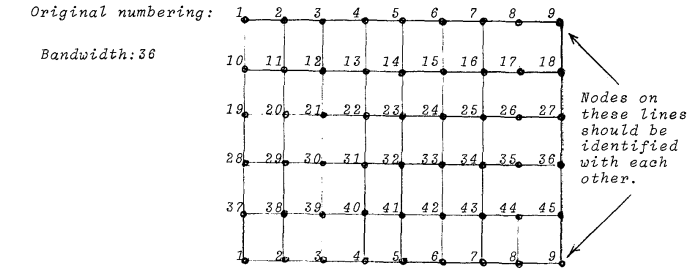
\includegraphics[width=0.49\linewidth]{figures/linear_cuthill-mckee_original.png}
    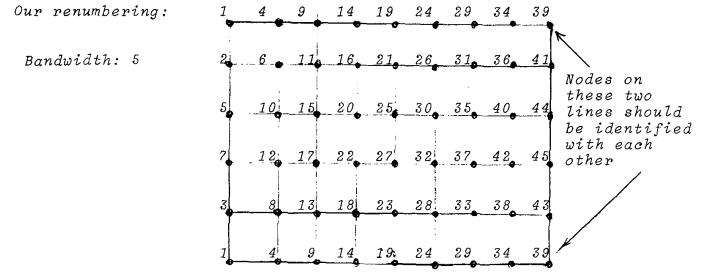
\includegraphics[width=0.49\linewidth]{figures/linear_cuthill-mckee_improved.png}
    \caption{Example from the original Cuthill--McKee paper~\cite{cuthill1969reducing}.}%
    \label{figure:linear_example_from_cuthill_mckee}
\end{figure}

